%% %% The fluid mass balance equation is solved in the current
%% %% configuration, i.e. (\ref{massbalcurr}) for $\iota = \mathrm{f}$, but 
%% %% mass balance for the solid collagenous phase is solved in the
%% %% reference configuration, i.e. (\ref{massbalance1}) for $\iota =
%% %% \mathrm{c}$. 

%% %% The balance of linear momentum
%% %% that we solve is (\ref{linearmombalance}) summed for $\iota =
%% %% \mathrm{c,f}$, with the constraint in (\ref{qrelation}) imposed.

%% \begin{figure}[ht]
%%   \centering
%%   \psfrag{BC}{\small Concentration boundary condition}
%%   \psfrag{RC}{\small Reduced concentration}
%%   \includegraphics[width=0.4\textwidth]
%%                   {images/elucidation/reference-boundary-conditions}
%%   \caption{Constant concentration boundary conditions in the reference
%%     configuration.} 
%%   \label{erroneous-bc}
%% \end{figure}

%% Relations (\ref{\ref{masssummationresult}}),
%% (\ref{momentumsummationresult}) and (\ref{energysummationresult})
%% relating the interaction terms are used to reduce the system of
%% equations when solving combined tissue-level problems

%%  In the numerical our numerical simulations that appear below in
%% Section~\ref{}, the numerical values used for
%% the parameters introduced in (\ref{wlcmeq}) are based on those in
%% \citet{kuhlremod05}.

%% Point to appendix, if it will exist.


%% \noindent{\bf Remark 4}: The constitutive relations
%% (\ref{stress-constrelI}) and (\ref{MIconstrel}) respectively
%% specify the partial stress, $\bP^\iota$, and flux, $\bM^\iota$, of
%% a species. The flux also implies the relative velocity,
%% $\bV^\iota$. The velocity of the solid phase, $\bV$ is obtained
%% from the local form of the balance of linear momentum for the
%% system (\ref{linmombalsys}). With all these quantities known, the
%% individual interaction forces between species,
%% $\rho^\iota_0\bq^\iota$, can be obtained from
%% (\ref{ballinmomrefI}). They are, however, not needed while solving
%% for the balance of linear momentum of the system.

%% The theory developed in Sections \ref{sect2}--\ref{sect5} has been
%% implemented in a computational formulation, retaining much of the
%% complexity of the coupled balance laws and constitutive relations.
%% For realistic soft tissue material parameters, the contribution of
%% the fluxes and interaction forces between species to the balance
%% of linear momentum of the composite tissue is negligible. This
%% simplification has been used. As a preliminary demonstration of
%% the theory\footnote{This numerical section has been included
%% mainly for completeness of this theoretical paper. A separate
%% paper, currently in preparation, will present the computational
%% formulation and contain a detailed examination of a number of
%% initial and boundary value problems for growth.}, we present a
%% computation of the coupled physics in the early stages of uniaxial
%% extension of a cylindrical soft tissue specimen. The motivation
%% for this model problem comes from our experimental model of
%% engineered, functional tendon constructs grown \emph{in vitro},
%% having the same cylindrical geometry. The experimental aspects of
%% our broad-based project on soft tissue growth are described
%% elsewhere \citep{Calve:04}. In addition to engineering
%% scaffold-less tendon constructs from neonatal rat fibroblast
%% cells, we have the ability to impose a range of mechanical,
%% chemical, nutritional and electrical stimuli on them and study the
%% tissue's response. Besides modelling these experiments, the
%% mathematical formulation described here presents researchers with
%% a vehicle for testing scenarios and framing hypotheses that can be
%% experimentally-validated in our laboratory, thereby driving the
%% experimental studies.

%% %\subsection{Boundary and initial conditions; coupled solution method}
%% %\label{}

%% Boundary conditions for mass transport consisted of the specified
%% fluid concentration at all external surfaces of the cylinder. This
%% value was fixed at $500\,\mathrm{kg.m}^{-3}$. With these boundary
%% conditions the fluid flux normal to surfaces of the specimen is
%% determined by solving the initial and boundary value problem. The
%% bottom planar surface was fixed in the $\be_3$ direction and a
%% displacement was applied at the top surface, also in the $\be_3$
%% direction, to give a nominal strain rate of
%% $0.05\,\mathrm{sec}^{-1}$ in the $\be_3$ direction. This is the
%% only mechanical load on the problem. Initial conditions were
%% $\rho_0^\mathrm{f}(\bX,0) =
%% 500\,\mathrm{kg.m}^{-3},\;\rho_0^\mathrm{s}(\bX,0) =
%% 500\,\mathrm{kg.m}^{-3}$, and for the mechanical problem,
%% $\bu(\bX,0) = \bzero,\,\bV(\bX,0) = \bzero$.

%% The coupled problem was solved by a staggered scheme based upon
%% operator splits
%% . The details 
%% will be presented in a future communication that will focus upon
%% computational aspects and numerical examples. Here we only mention
%% that the staggered scheme consists of identifying the displacement
%% and species concentrations as primitive variables associated with
%% the mechanical and mass transport problems. The mechanical problem
%% is solved holding the concentrations fixed. The resulting
%% displacement field is then held constant to solve the mass
%% transport problem. The transient solution is obtained for
%% mechanics using energy-momentum conserving schemes
%% \citep{SimoTarnow:1992b,SimoTarnow:1992a,Gonzalezphd:1996}, and
%% for mass transport using the Backward Euler Method. Hexahedral
%% elements are employed, combined with nonlinear projection methods
%% \citep{simotaylorpister:85} to treat the near-incompressibility
%% imposed by the fluid. The numerical formulation has been
%% implemented within the nonlinear finite element program, FEAP
%% \citep{feapmanual}.

%% --------------



%% Its specialization to the case discussed in this section is straighforward. The particular
%% choice of primitive unknowns used in this section can be shown to ensure unconditional stability
%% of this operator split for parabolic 
%% uid transport equations that are equivalent to our formulation,
%% 2Fickean diusion manifests itself as a concentration gradient-driven 
%% ux. Even in the absence of Fickean diusion, a
%% concentration gradient 
%% ux remains, since the 
%% uid stress is concentration-dependent.
%% 6
%% and coupled with nite strain elasticity (Armero, 1999). This was borne out in our computations, with
%% somewhat slow convergence with respect to number of passes, due to the strong coupling of this problem.
%% (One pass is completed when all equations have been solved once.) In Section 5 we demonstrate how
%% this analysis can be extended to the reformulation of the growth problem, by solution of the detailed
%% solid and 
%% uid momentum balance equations, that is being advocated in this proposal.

%% Identifying the displacement fields, $\bu$, and
%% the concentration fields, $\rho^{\iota}$, as primitive variables
%% associated with the mechanical and mass transport problems, each
%% equation is solved for their respective variable holding all other
%% variables fixed, in turn. 

%%  the
%% balance of momentum is solved holding the concentrations fixed, and
%% the resulting displacement field is then held constant to solve the
%% balance of mass equations. Convergence of the system of equations is
%% attained when the solution of each set of equations has converged to
%% within a 


%% %% However, we will not attempt detailed descriptions of
%% %% experiments, choosing to focus 
%% %% instead on results that can be directly related to the models. A more
%% %% detailed comparison with experiments is forthcoming in a separate
%% %% communication.


%% {\bf Unbounded pinching problem}

%% \subsection{Fluxes from different driving forces}
%% \label{flux-driving-forces}

%% The following contour plots represent the stress, and various
%% contributions to the total flux in the early stages of loading of
%% the model problem. Symmetry has been employed to model a single
%% quadrant of the cylinder.

%% The longitudinal stress, $\sigma_{33}$ in Figure \ref{stressfig}
%% arises from the stretch and the evolution in concentration.
%% \begin{figure}[!hpt]
%% \begin{minipage}[t]{7.5cm}
%% {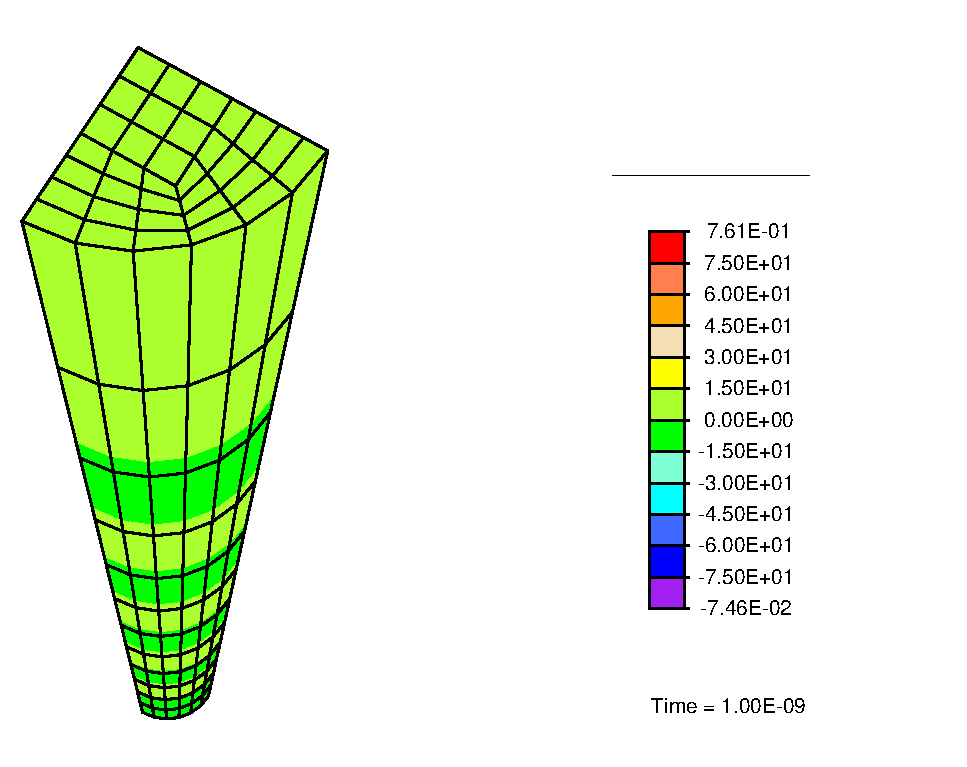
\includegraphics[width=7.5cm]{images/examples/lagrangian/preliminary/S33-1}} \hskip 3cm (a) 
%% \end{minipage}
%% \begin{minipage}[t]{7.5cm}
%% {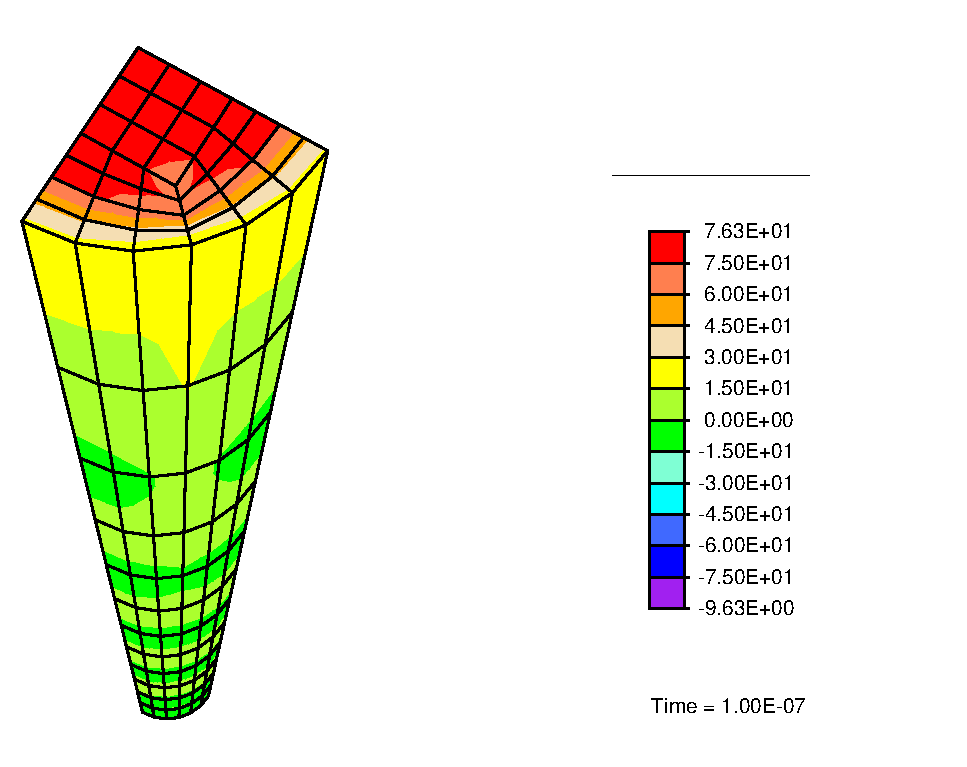
\includegraphics[width=7.5cm]{images/examples/lagrangian/preliminary/S33-100}} \hskip 3cm (b)
%% \end{minipage}
%% \caption{Longitudinal Cauchy stress, $\sigma_{33}$ (Pa) at $1
%% \,\mathrm{nanosec.}$ and $100\,\mathrm{nanosec.}$ after the
%% beginning of loading.} \label{stressfig}
%% \end{figure}

%% \begin{figure}[!hpt]
%% \begin{minipage}[t]{7.5cm}
%% {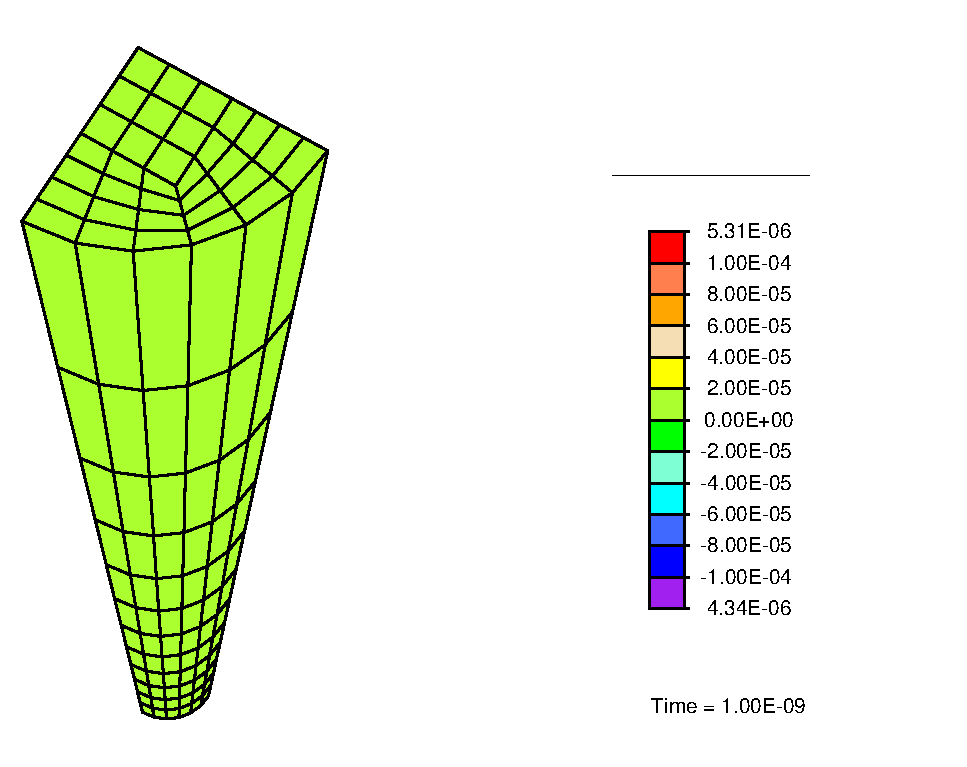
\includegraphics[width=7.5cm]{images/examples/lagrangian/preliminary/M1-1}} \hskip 3cm (a)
%% \end{minipage}
%% \begin{minipage}[t]{7.5cm}
%% {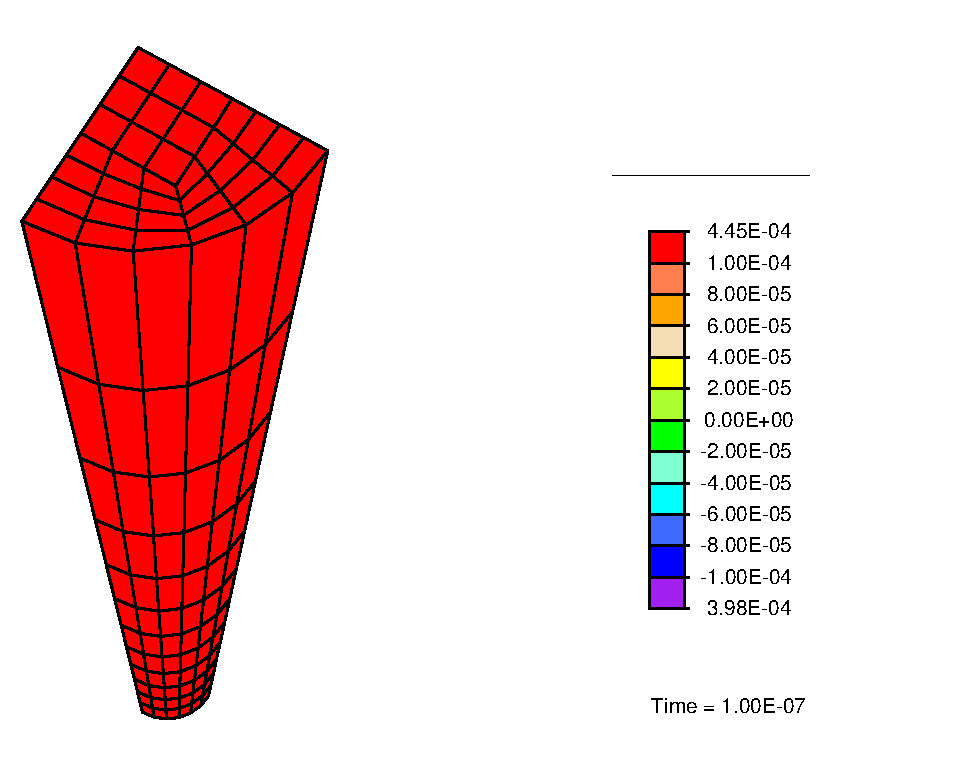
\includegraphics[width=7.5cm]{images/examples/lagrangian/preliminary/M1-100}} \hskip 3cm (b)
%% \end{minipage}
%% \caption[Stress gradient-driven flux]{Stress gradient-driven flux
%% ($\mathrm{kg.m}^{-2}\mathrm{sec}$) in the $\be_3$ direction at $1
%% \,\mathrm{nanosec.}$ and $100\,\mathrm{nanosec.}$ after the
%% beginning of loading. The positive values indicate an upward flux
%% corresponding to a tensile $\sigma_{33}$ wave travelling
%% downwards.} \label{M1fig}
%% \end{figure}

%% \begin{figure}[!hpt]
%% \begin{minipage}[t]{7.5cm}
%% {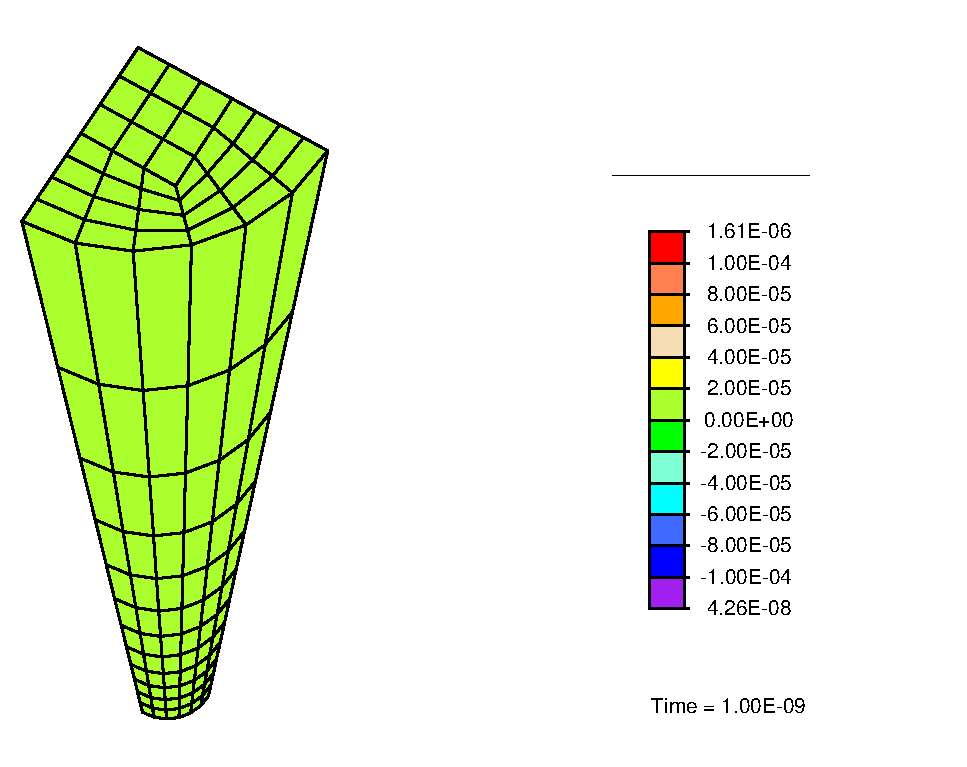
\includegraphics[width=7.5cm]{images/examples/lagrangian/preliminary/M2-1}} \hskip 3cm (a)
%% \end{minipage}
%% \begin{minipage}[t]{7.5cm}
%% {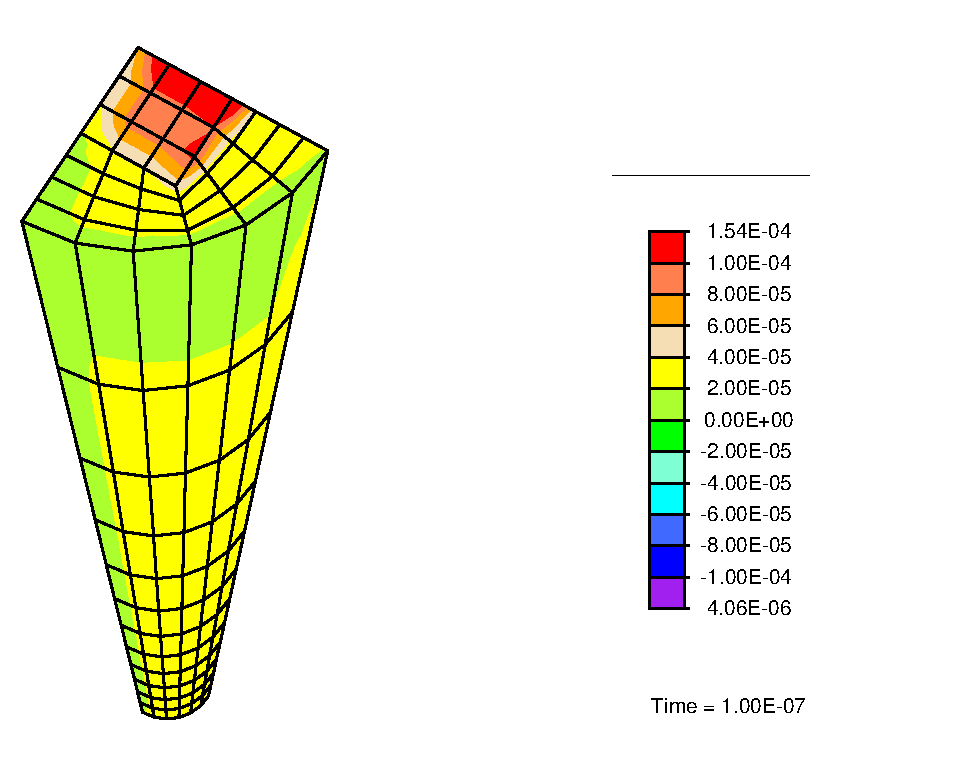
\includegraphics[width=7.5cm]{images/examples/lagrangian/preliminary/M2-100}} \hskip 3cm (b)
%% \end{minipage}
%% \caption{Internal energy gradient-driven flux,
%% ($\mathrm{kg.m}^{-2}\mathrm{sec}$) in the $\be_3$ direction at $1
%% \,\mathrm{nanosec.}$ and $100\,\mathrm{nanosec.}$ after the
%% beginning of loading. The positive values indicate an upward flux.
%% This corresponds to a lower energy near the top of the cylinder as
%% the tensile stress ($\sigma_{33}$) wave travels downward and
%% relaxes some of the strain energy of contraction.} \label{M2fig}
%% \end{figure}

%% \begin{figure}[!hpt]
%% \begin{minipage}[t]{7.5cm}
%% {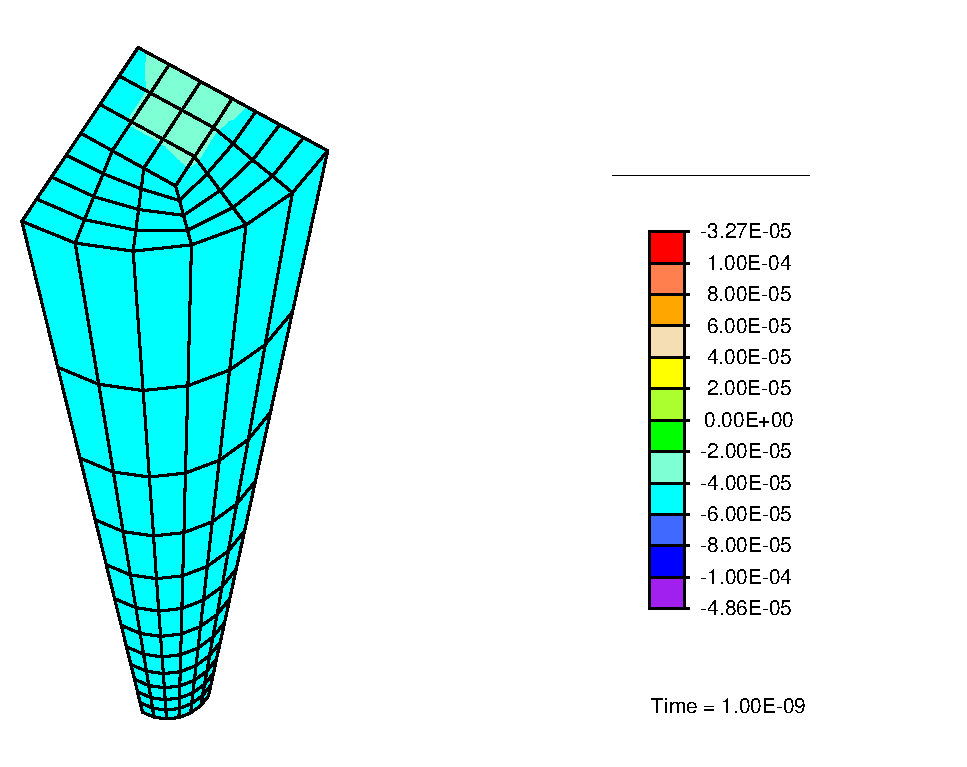
\includegraphics[width=7.5cm]{images/examples/lagrangian/preliminary/M3-1}} \hskip 3cm (a)
%% \end{minipage}
%% \begin{minipage}[t]{7.5cm}
%% {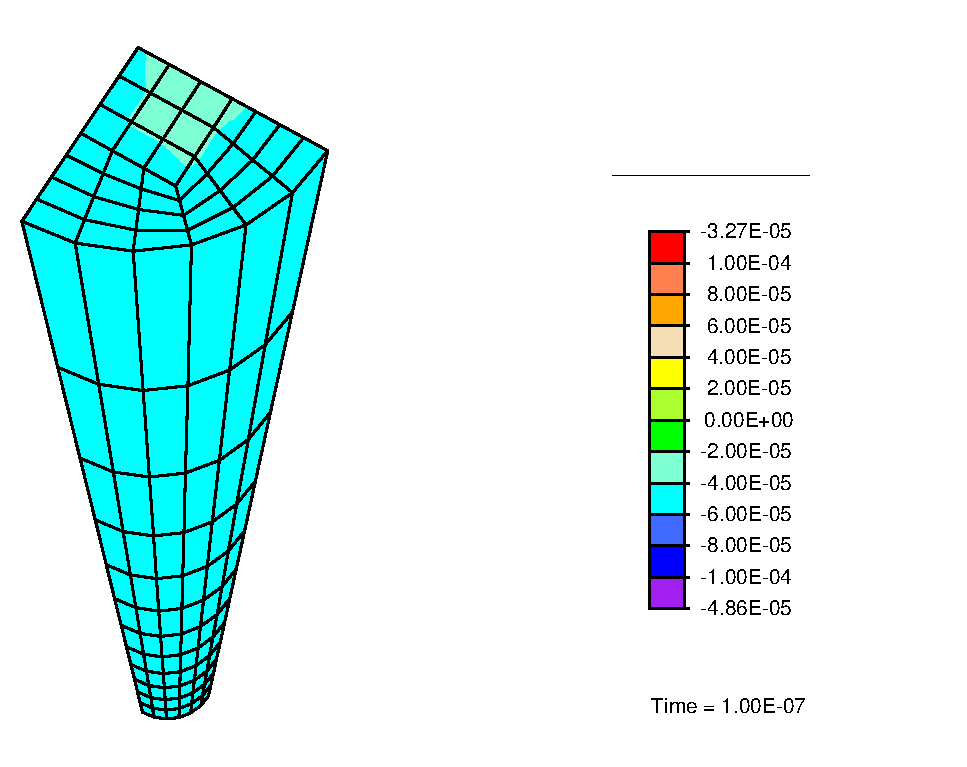
\includegraphics[width=7.5cm]{images/examples/lagrangian/preliminary/M3-100}} \hskip 3cm (b)
%% \end{minipage}
%% \caption{Gravity-driven flux ($\mathrm{kg.m}^{-2}\mathrm{sec}$) in
%% the $\be_3$ direction at $1 \,\mathrm{nanosec.}$ and
%% $100\,\mathrm{nanosec.}$ after the beginning of loading. The
%% negative values indicate a downward flux, due to the action of
%% gravity.} \label{M3fig}
%% \end{figure}

%% \begin{figure}[!hpt]
%% \begin{minipage}[t]{7.5cm}
%% {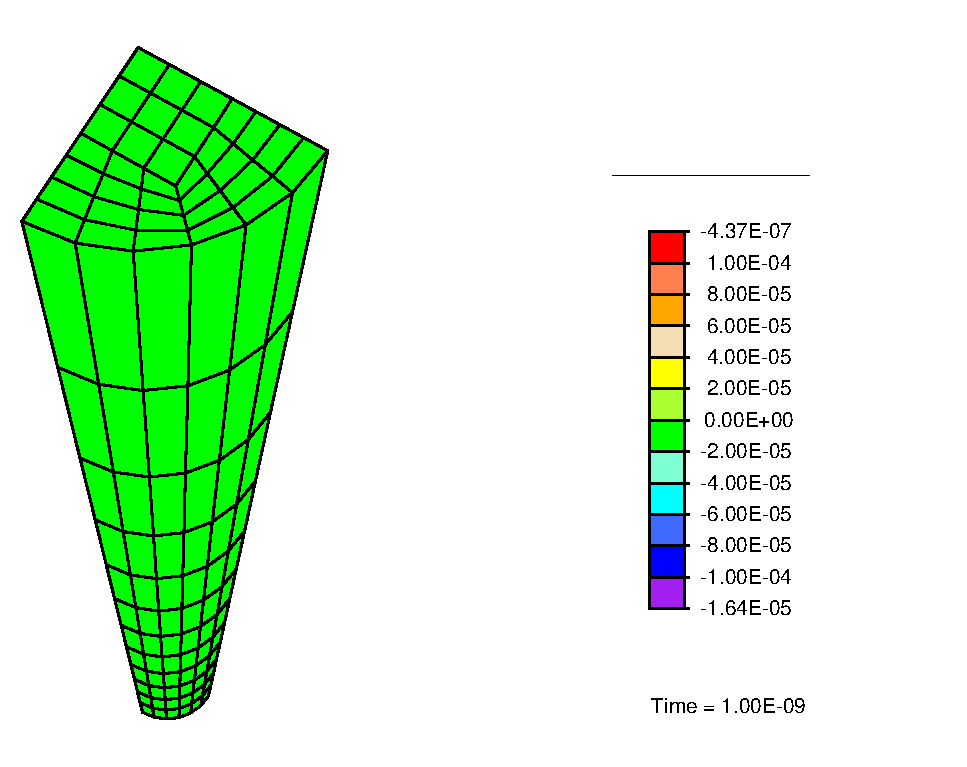
\includegraphics[width=7.5cm]{images/examples/lagrangian/preliminary/M4-1}} \hskip 3cm (a)
%% \end{minipage}
%% \begin{minipage}[t]{7.5cm}
%% {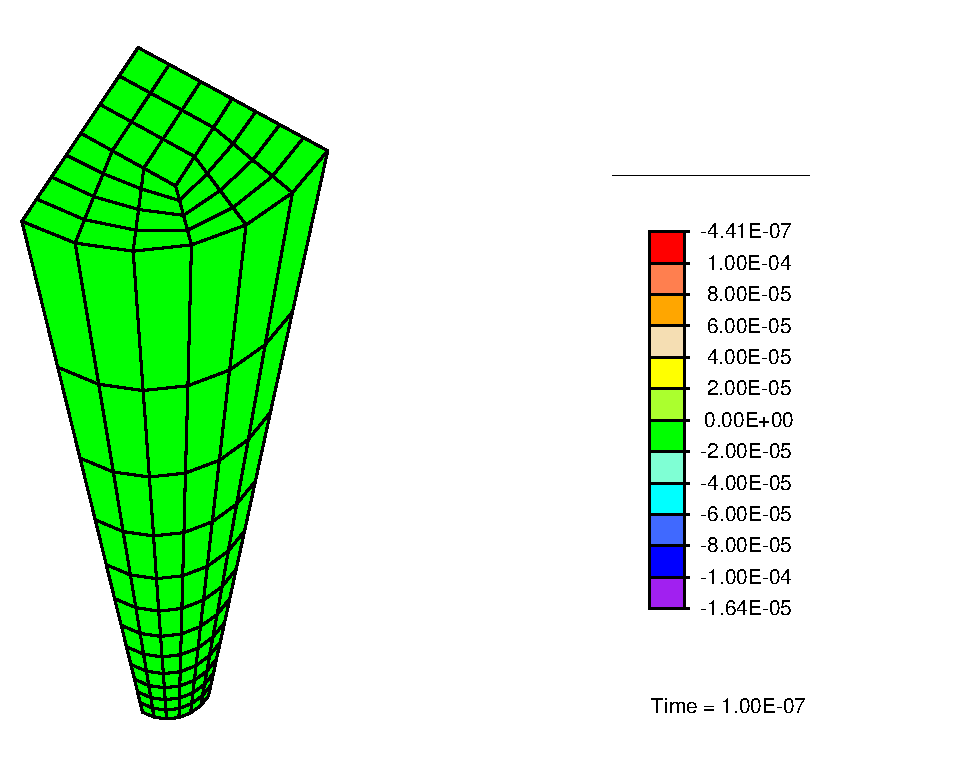
\includegraphics[width=7.5cm]{images/examples/lagrangian/preliminary/M4-100}} \hskip 3cm (b)
%% \end{minipage}
%% \caption{Inertia-driven flux ($\mathrm{kg.m}^{-2}\mathrm{sec}$) in
%% the $\be_3$ direction at $1 \,\mathrm{nanosec.}$ and
%% $100\,\mathrm{nanosec.}$ after the beginning of loading. The
%% negative values indicate a downward flux as the tissue accelerates
%% upward.} \label{M4fig}
%% \end{figure}

%% \begin{figure}[!hpt]
%% \begin{minipage}[t]{7.5cm}
%% {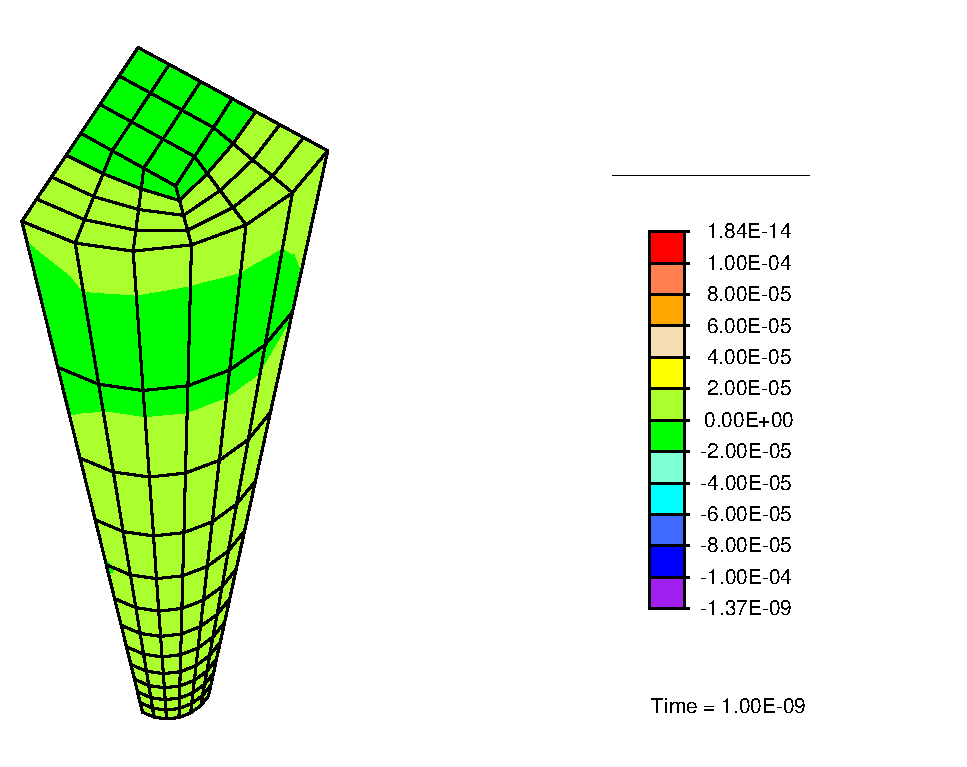
\includegraphics[width=7.5cm]{images/examples/lagrangian/preliminary/M5-1}} \hskip 3cm (a)
%% \end{minipage}
%% \begin{minipage}[t]{7.5cm}
%% {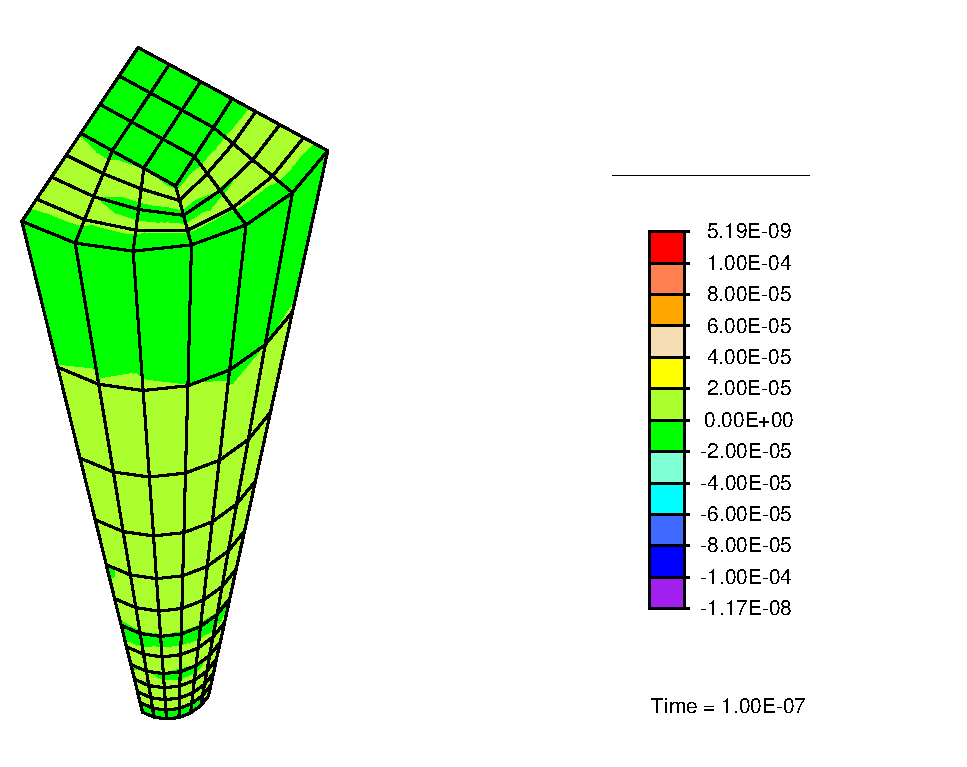
\includegraphics[width=7.5cm]{images/examples/lagrangian/preliminary/M5-100}} \hskip 3cm (b)
%% \end{minipage}
%% \caption{Concentration gradient-driven flux
%% ($\mathrm{kg.m}^{-2}\mathrm{sec}$) in the $\be_3$ direction at $1
%% \,\mathrm{nanosec.}$ and $100\,\mathrm{nanosec.}$ after the
%% beginning of loading. Note that the maximum and minimum values are
%% many orders of magnitude lower than for the other flux
%% contributions reported above. This is a demonstration of mechanics
%% influences dominating diffusion over the classical concentration
%% gradient contribution.} \label{M5fig}
%% \end{figure}

%% \begin{figure}[!hpt]
%% \begin{minipage}[t]{7.5cm}
%% {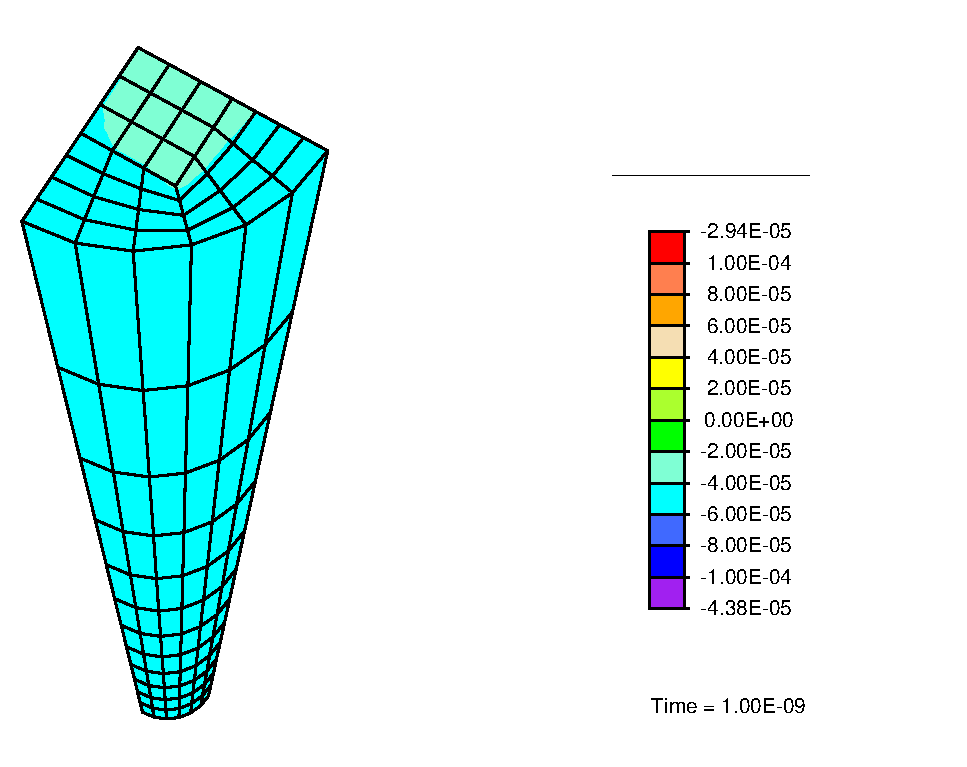
\includegraphics[width=7.5cm]{images/examples/lagrangian/preliminary/M-1}} \hskip 3cm (a)
%% \end{minipage}
%% \begin{minipage}[t]{7.5cm}
%% {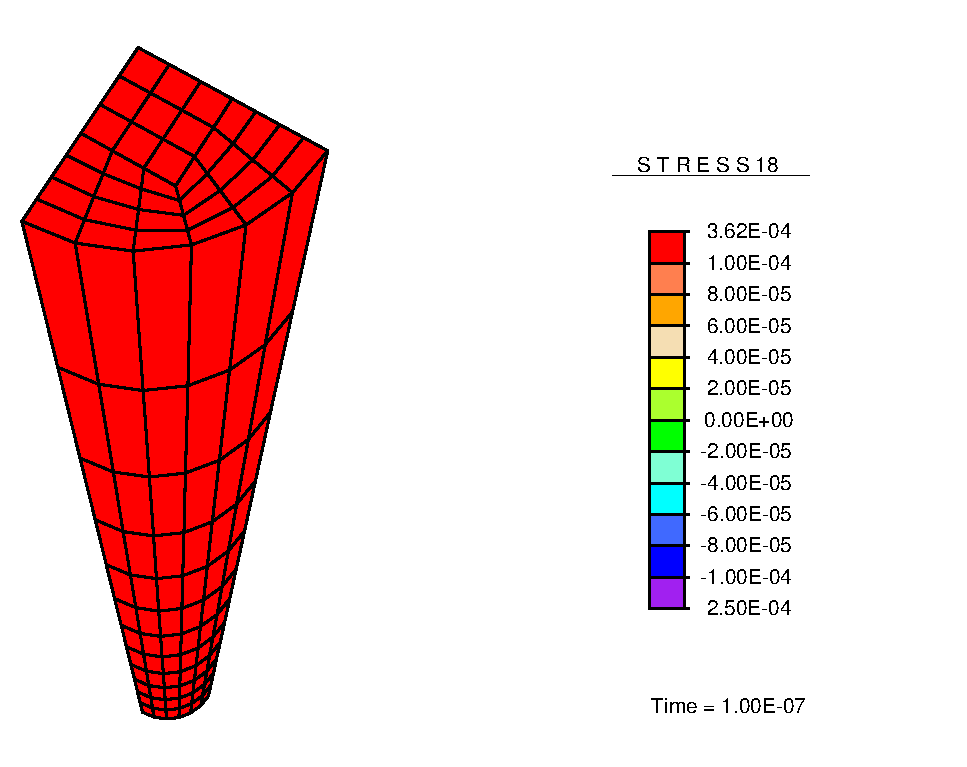
\includegraphics[width=7.5cm]{images/examples/lagrangian/preliminary/M-100}} \hskip 3cm (b)
%% \end{minipage}
%% \caption{Total flux ($\mathrm{kg.m}^{-2}\mathrm{sec}$) in the
%% $\be_3$ direction at $1 \,\mathrm{nanosec.}$ and
%% $100\,\mathrm{nanosec.}$ after the beginning of loading. The
%% positive values indicate an upward flux, dominated by the stress
%% gradient driven contribution.} \label{Mfig}
%% \end{figure}

%% The flux contributions in Figures \ref{M1fig}--\ref{Mfig} can be
%% summarized as follows: The fluid flux is dominated by the
%% contribution from the stress gradient in the $\be_3$ direction.
%% The latter arises as the stress ($\sigma_{33}$) wave of tension
%% travels down the cylinder in the first few microseconds after
%% application of the load (the time taken to travel the length of
%% the cylinder is $12 \,\mu\mathrm{sec}$). Additionally, as the
%% fluid concentration changes due to the flux, it causes a further
%% change in the stress (Section \ref{sect5}). Other flux terms are
%% qualitatively sensible; i.e., their directions are consistent with
%% the physics of the problem, as argued in each of the figure
%% captions\footnote{In order to compare the flux contributions, they
%% have all been plotted on the same scale: $-1\times
%% 10^{-4}--1\times 10^{-4} \,\mathrm{kg.m}^{-2}\mathrm{sec}$.
%% However the plots also show the maximum and minimum field values
%% at the top and bottom of the legend bars. These values represent a
%% better comparison of the relative flux magnitudes.}. There is some
%% loss of axial symmetry in a few of the plots due to the coarseness
%% of the finite element mesh for this example. It appears that
%% spatial oscillations in the solution lead to a further loss of
%% symmetry in Figures \ref{M2fig}b--\ref{M3fig}b and \ref{Mfig}a.
%% These oscillations arise due to large and dominant advective
%% terms, and need to be remedied by stabilized finite element
%% methods. Here, we only aim to demonstrate that various driving
%% forces for mass transport are in agreement with their theoretical
%% underpinnings in the paper. The resorption of the solid phase is
%% shown indirectly in Figure \ref{Pifig}. A positive fluid source,
%% $\Pi^\mathrm{f}$, means that $\Pi^\mathrm{s} < 0$. Since
%% $\Pi^\mathrm{s}$ is the only term balancing
%% $\partial\rho_0^\mathrm{s}/\partial t$ [see (\ref{massballocA})],
%% it follows that $\partial\rho_0^\mathrm{s}/\partial t < 0$.

%% \begin{figure}[!hpt]
%% \begin{minipage}[t]{7.5cm}
%% {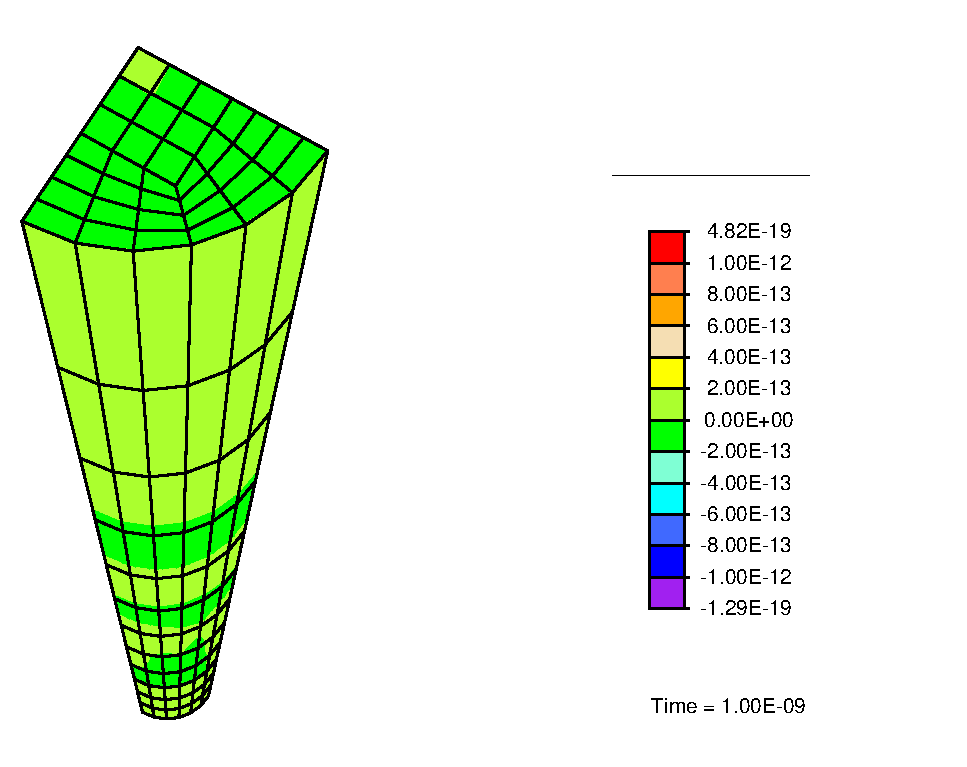
\includegraphics[width=7.5cm]{images/examples/lagrangian/preliminary/Pi-1}} \hskip 3cm (a)
%% \end{minipage}
%% \begin{minipage}[t]{7.5cm}
%% {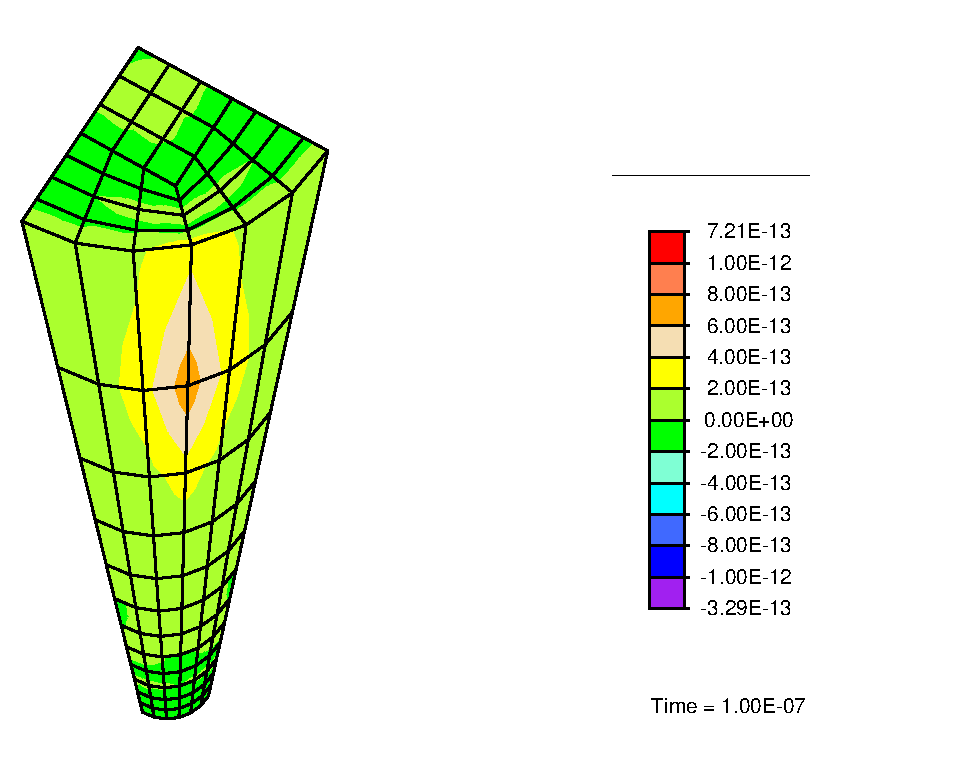
\includegraphics[width=7.5cm]{images/examples/lagrangian/preliminary/Pi-100}} \hskip 3cm (b)
%% \end{minipage}
%% \caption{Rate of fluid production, $\Pi^\mathrm{f}$
%% ($\mathrm{kg.m}^{-3}.\mathrm{sec}^{-1}$), at $1
%% \,\mathrm{nanosec.}$ and $100\,\mathrm{nanosec.}$ after the
%% beginning of loading. The positive values indicate that the local
%% fluid concentrations have fallen below their initial values.}
%% \label{Pifig}
%% \end{figure}

%The mixing entropy of fluid in the mixture with collagen is
%written as $\eta_{\mathrm{mix}}^{f} = -\frac{k}{\sM^\mathrm{f}}
%\mathrm{log} (\frac{\rho^\mathrm{f}} {\rho})$, where
%$\sM^\mathrm{f}$ is the molecular weight of the fluid.

%\subsection{Using the appropriate configuration}
%\label{appropriate-configuration}


%% \subsubsection{Upper bound model}
%% \label{upper-bound}

%% \subsubsection{Lower bound model}
%% \label{lower-bound}


%% \begin{figure}[!hpt]
%% \centering
%% 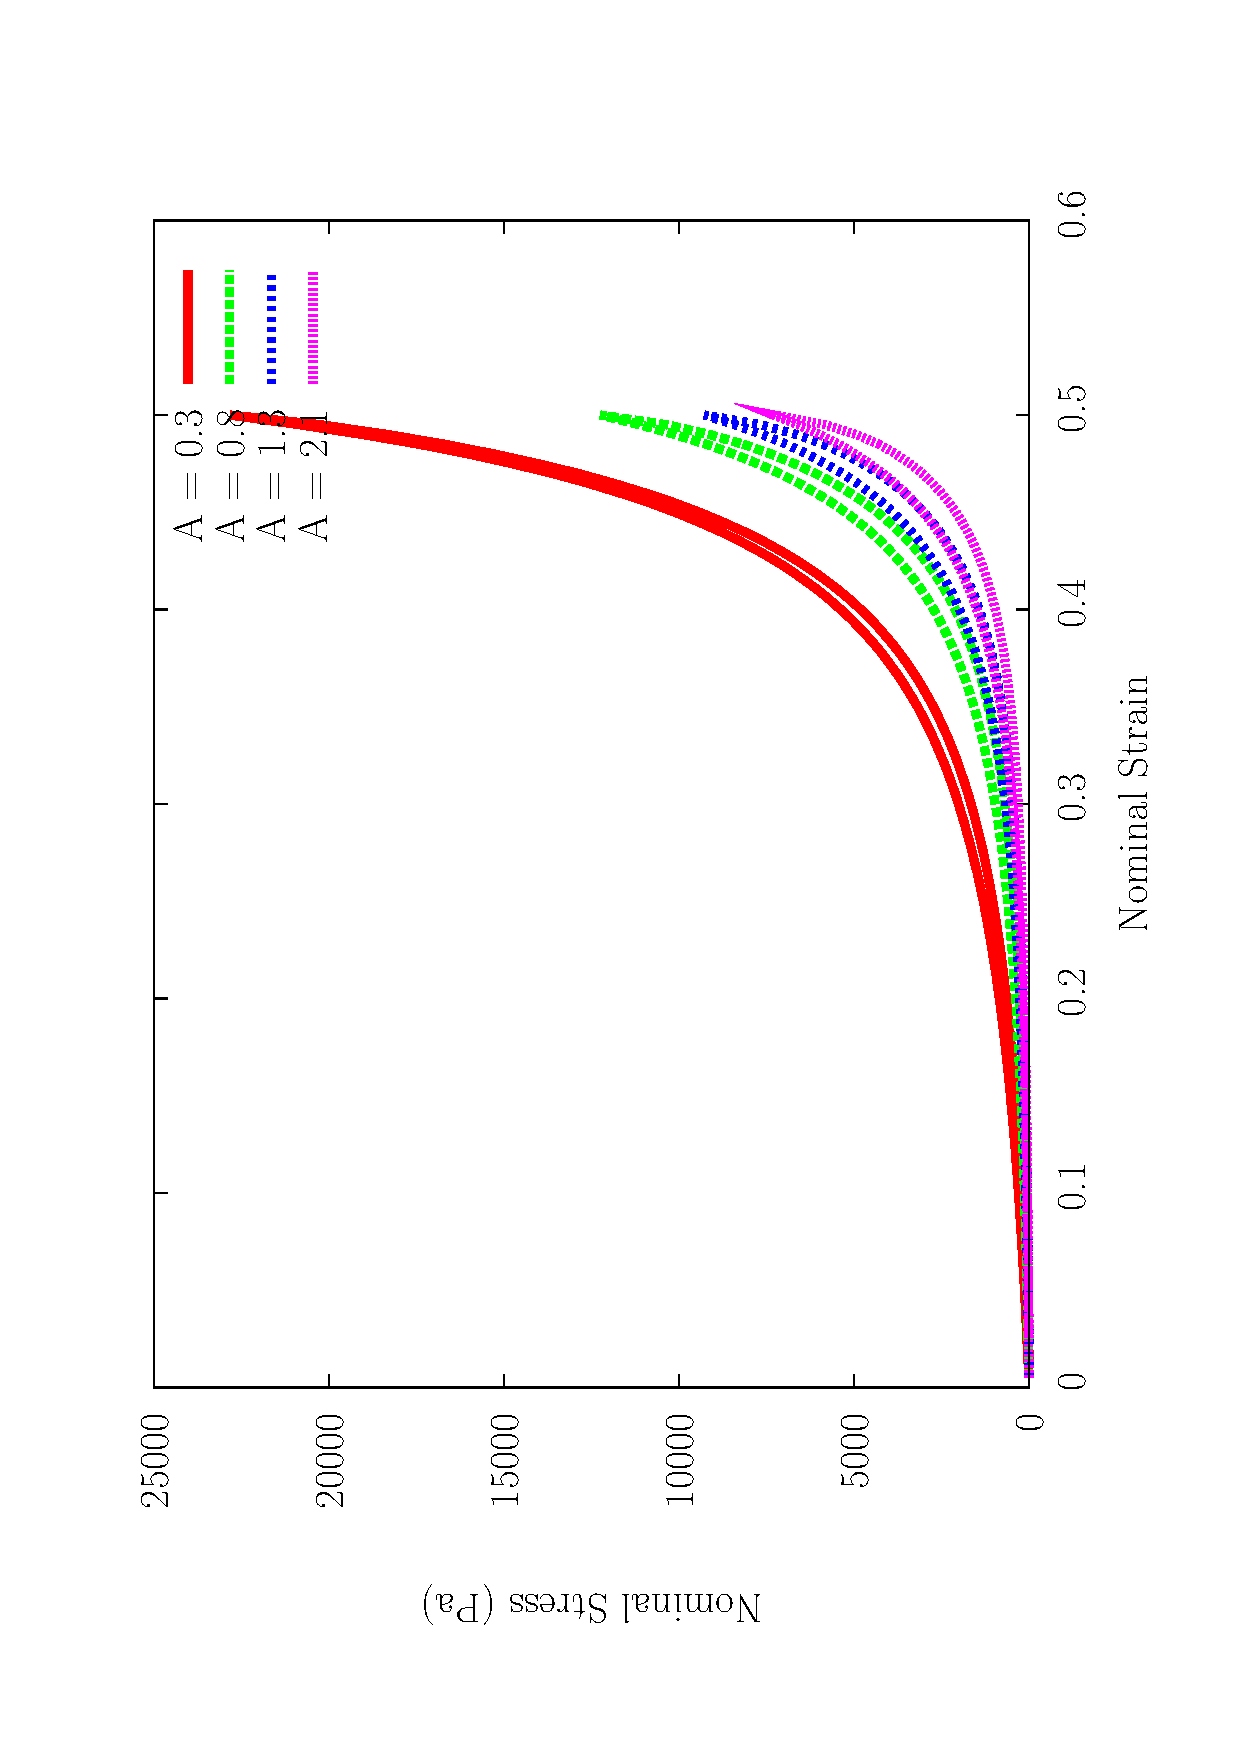
\includegraphics[angle=270,width=0.6\textwidth]{images/examples/lagrangian/cyclic/parametric-study}
%% \caption{Varying A}
%% \label{parametric-study}
%% \end{figure}

%% \begin{figure}[!hpt]
%% \centering
%% 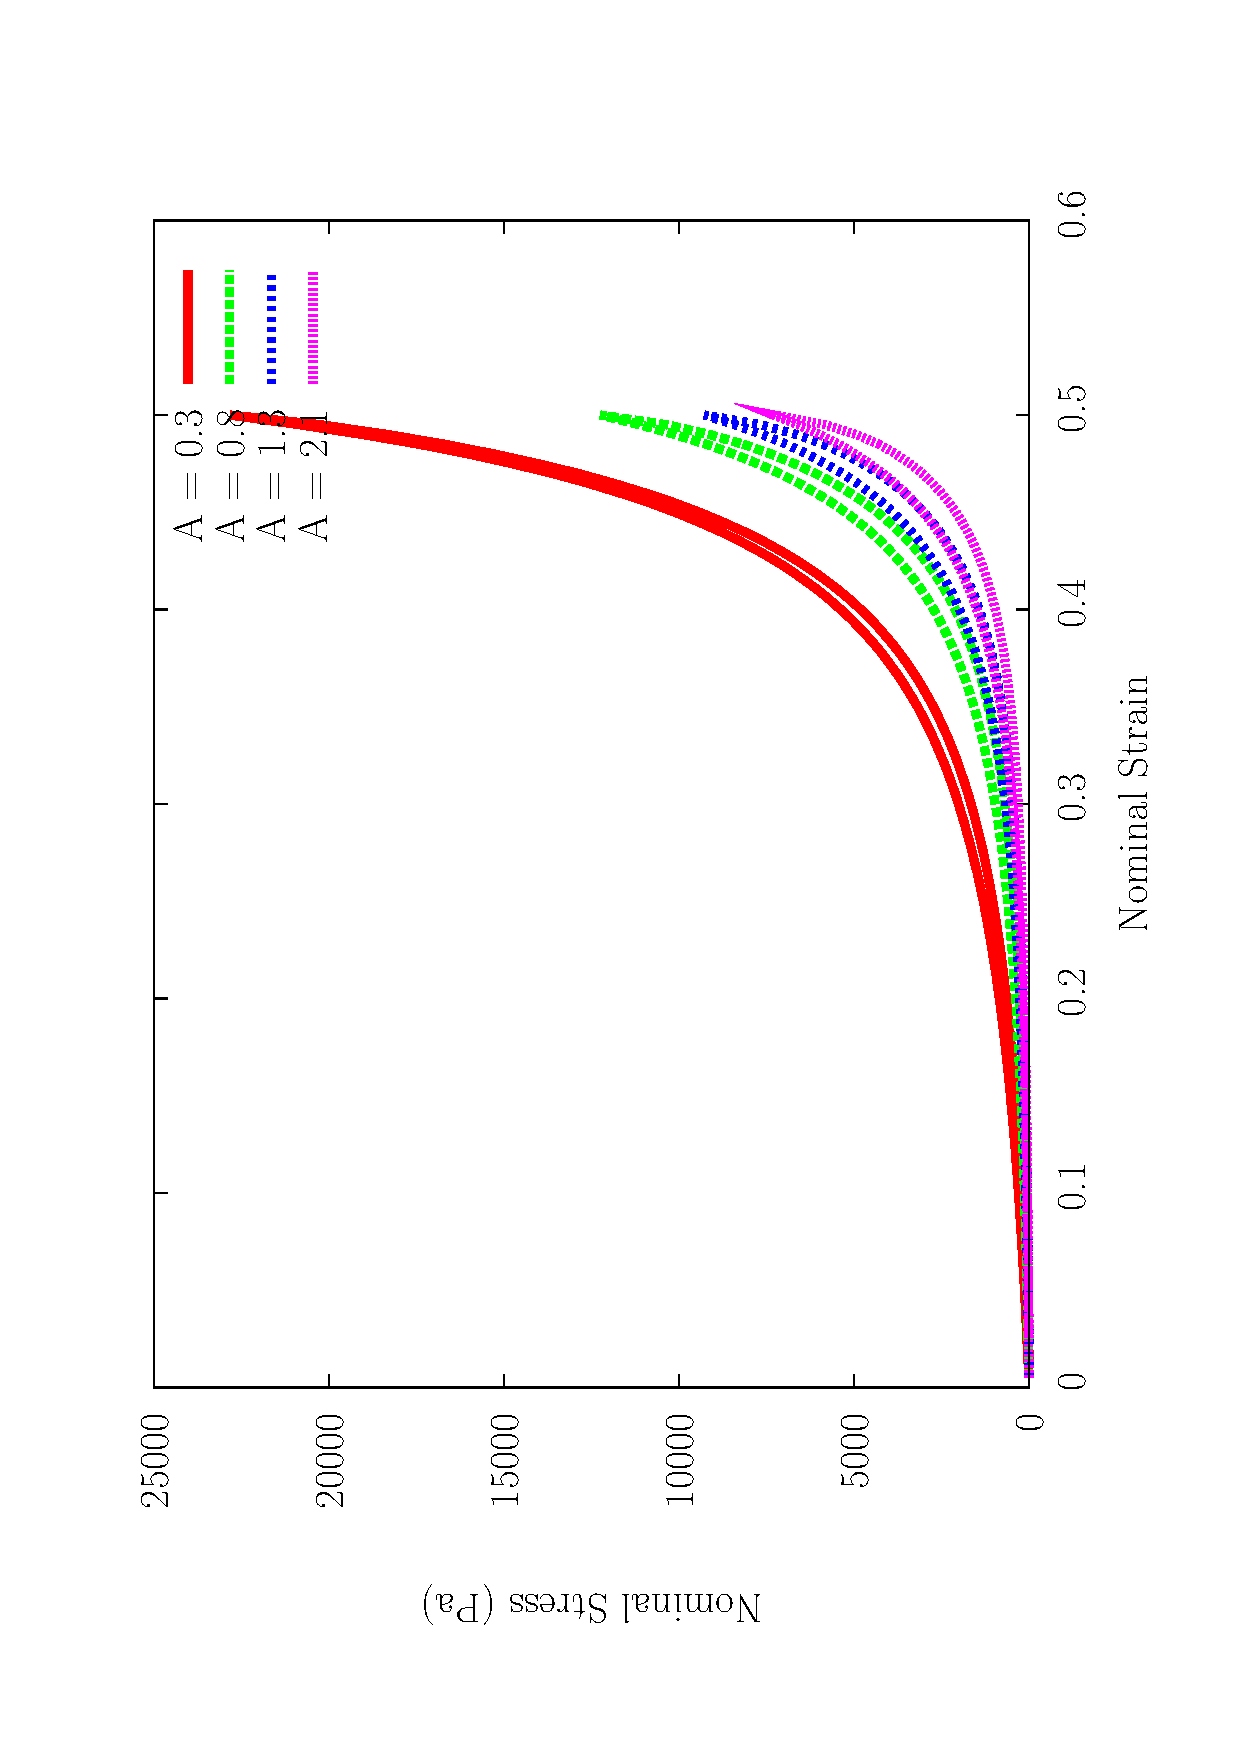
\includegraphics[angle=270,width=0.6\textwidth]{images/examples/lagrangian/cyclic/parametric-study}
%% \caption{Load-unload cycle}
%% \label{cyclic-load}
%% \end{figure}


% \multicolumn{1}{|l}{Parameter (Symbol)} & {|l}Value &
      % Units\\ \hline

%% \section{Extension to modelling wound healing}
%% \label{wound-healing-example}

%% \todo{Flesh this example out or remove it.}

%% \begin{figure}[!hpt]
%% \centering
%% \includegraphics[width=0.8\textwidth]
%%                {images/experiments/healing-damaged-ligament} 
%% \caption{The recovery of a damaged ligament.}
%% \label{healing-damaged-ligament}
%% \end{figure}

%% There is experimental evidence to suggest that during wound healing,
%% newly-de\-po\-sit\-ed collagen fibres are found to align with the
%% applied stress whereas under unstressed conditions, they are deposited
%% isotropically \citep{Provenzanoetal:2003}.

%% \begin{equation}
%% \Pi^\mathrm{c} = \alpha\ k^\mathrm{f}(\rho_0^\mathrm{f} -
%% \rho_{0_\mathrm{ini}}^\mathrm{f}),
%% \label{cell-signalling-source}
%% \end{equation}

%% Contains two phases. Portion of solid initially ``broken.'' --
%% $400$~\mbox{kg.m}$^{-3}$ in the damaged regions and
%% 500~\mbox{kg.m}$^{-3}$ everywhere else in the domain. Fluid initially
%% 400~\mbox{kg.m}$^{-3}$ in the domain and 500~\mbox{kg.m}$^{-3}$ in the
%% nutrient-rich bath $\Rightarrow$ fluid and nutrients rush in, as in
%% the swelling problem.

%% $\alpha$ is a cell-signalling parameter which
%% drives preferential growth in damaged regions mimicking the
%% availability of cells in those regions. It's currently a simple
%% switch, $\alpha = 1$ if
%% $\rho_0^{\mathrm{c}}<500$~\mbox{kg.m}$^{-3}$ and $\alpha = 0$
%% otherwise. Same $k^\mathrm{f}$ as before.

%% Time starts, fluid flows in like the swelling problem, but unlike the
%% swelling problem growth only takes place in damaged regions. The
%% process is carried out under load, and under no load and the numerical
%% experiment is run until $\alpha=0$ everywhere, meaning the collagen
%% concentration is back to $\rho_0^{\mathrm{c}}=500$~\mbox{kg.m}$^{-3}$
%% at all points in the tissue, indicating a ``fully-healed'' tissue.

%% Newly deposited collagen is modelled as a ``different'' material in the
%% code. It is the same as the old material, but with but with material
%% constants that depend on the stress state upon deposition. Under load,
%% it's 

%% %of scars are the result of the body overproducing collagen, which causes the scar to be raised above the surrounding skin. Hypertrophic scars take the form of a red raised lump on the skin, but do not grow beyond the boundaries of the original wound, and they often improve in appearance after a few years

%% %% chemo-mechanical
%% %% coupling is described in \cite{Provenzanoetal:2003}.



%% \begin{figure}[!hpt]
%% \centering
%% \includegraphics[width=0.8\textwidth]
%%                 {images/examples/lagrangian/healing/full-skin-mesh} 
%% \caption{The computational mesh representing the tissue.}
%% \label{healing-skin-mesh}
%% \end{figure}

%% \begin{figure}[!hpt]
%% \centering
%% \includegraphics[width=0.8\textwidth]
%%                 {images/examples/lagrangian/healing/damaged-region} 
%% \caption{A section of the mesh highlighting the damaged region.}
%% \label{healing-damaged-region}
%% \end{figure}

%% \begin{figure}[!hpt]
%% \centering
%% \includegraphics[width=0.8\textwidth]
%%                 {images/examples/lagrangian/healing/healed-vertical-displacement} 
%% \caption{Vertical displacement upon loading after healing under no external load.}
%% \label{healing-vertical-displacement}
%% \end{figure}

%% \begin{figure}[!hpt]
%% \centering
%% \includegraphics[width=0.8\textwidth]
%%                 {images/examples/lagrangian/healing/healed-vertical-stress} 
%% \caption{Vertical stress upon loading after healing under no external load.}
%% \label{healing-vertical-stress}
%% \end{figure}
